% Copyright (C) 2018 by latexstudio <http://www.latexstudio.net>
%
% This program is free software: you can redistribute it and/or modify
% it under the terms of the GNU General Public License as published by
% the Free Software Foundation, either version 3 of the License, or
% (at your option) any later version.
%
% This program is distributed in the hope that it will be useful,
% but WITHOUT ANY WARRANTY; without even the implied warranty of
% MERCHANTABILITY or FITNESS FOR A PARTICULAR PURPOSE.  See the
% GNU General Public License for more details.
%
% You should have received a copy of the GNU General Public License
% along with this program.  If not, see <http://www.gnu.org/licenses/>.
%

\section{文档编辑}


\faq{\LaTeXTeX{} 教程}{latex-tex-tutorial}
lshort-zh 是一本比较薄的针对中文用户的 \LaTeX{} 入门教程,该教程已在发行版中,用户可以在命令行中执行
\begin{verbatim}
  texdoc lshort-zh
\end{verbatim}
来查阅。 \LaTeX wikibook 是
% \href{https://www.latex-project.org/help/books/}{https://www.latex-project.org/}
\url{https://www.latex-project.org/help/books/} 中列出的 \TeX{} and \LaTeX{} Books 之一,用户可访问
\url{https://en.wikibooks.org/wiki/LaTeX} 进行查阅。
除此之外,用户还可以购买胡伟、刘海洋等编著书籍,这里不再赘述。


\faq{关于 \LaTeX{} 的书籍}{latex-books}
\begin{itemize}
  \item \LaTeX{} 入门,刘海洋, 电子工业出版社;
  \item \LaTeX{2$\varepsilon$} 完全学习手册(第 2 版),胡伟,清华大学出版社;
  \item \LaTeX{} 入门与提高(第二版) ,陈志杰等,高等教育出版社(注:此书出版逾十年,部分内容已经过时);
  \item \LaTeX{} Beginner's Guide, Stefan Kottwit, Packt Publishing.
\end{itemize}


\faq{\LaTeX{} 支持中文有哪些方式,如何选择}{latex-chinese-how-to-choose}
历史上,\LaTeX{} 支持中文的方式包括中西文点点通、天元、CCT、CJK 等。目前流行的方式是使用 \CTeX{} 宏集,详情请见
\url{https://mirrors.tuna.tsinghua.edu.cn/CTAN/language/chinese/ctex/ctex.pdf}


\faq{关于教程,用户比较容易获取的有两个:lshort 和 \LaTeX{} wikibook。}{lshort-latex-wikibook}


\faq{关于\TeX{}, Plain \TeX{} 及相关书籍}{tex-plain-tex-books}


\faq{关于类型的书籍}{kind-related-books}


\faq{关于其他TeX相关事项的书籍}{other-tex-books}


\faq{工具包文档}{package-document}
每个工具包自带的文档是最全面最权威的文档,一般可以通过 texdoc 
命令+工具包名的方式找到相应工具包的文档。
一些常用的工具包有不少爱好者写了自己使用过程中的经验,也可以找来看看。


\faq{可免费提供的 \LaTeXTeX{} 书籍}{free-latex-tex-books}
\begin{itemize}
  \item \LaTeX{} 常用数学符号
  \item \LaTeX{} Note 包太雷
  \item 一份不太简短的 \LaTeX{2e} 介绍
  \item \TeX{} Live 指南 2018
\end{itemize}


\faq{获取在线帮助}{gain-online-help}
一般资料可以去 wikibook 上面查询,网址是
\url{https://en.wikibooks.org/wiki/LaTeX}。
提问可以先到 \LaTeX{} Stack Exchange 看看,网址是
\url{https://tex.stackexchange.com/}。


\faq{如何提出问题}{how-to-ask-questions}

在问问题的时候,要先自己尝试,先问自己如何解决,清晰有效的组织自己想问的问题,究竟想表达什么?没有人会为你不知所谓的问题浪费时间,就算有人愿意理你,也会因为你的问题不清晰甚至完全无效的问题而伤透脑筋,为了自己,也为了别人,建议大家可以参考下\href{https://www.jianshu.com/p/f96aa7f7bf59}{《提问的艺术》}这篇文字,清晰有效的提出自己的问题。迷你范例(MWE)是为别人帮助解决你的问题提供最大化便利的有效手段之一。

最后,需要强调的是,我们愿意在我们的能力范围内为你的问题进行讨论,尽全力帮你解决问题,但这并不是我们的义务,应当尊重别人拒绝提供的权利。另外,在 QQ 群提出问题所使用的代码最好代码粘贴的网站,如
\href{https://paste.ubuntu.com/}{Ubuntu Pastebin}
暂存,避免刷屏,影响效率。


\faq{如何制作一个迷你范例(MWE)}{how-to-make-MWE}
迷你范例即最小工作示例,英文简称 MWE,以下内容摘自刘海洋的《\LaTeX{} 入门》。

最小工作示例就是一个精简到最小长度的、可以说明所需问题的 \TeX{} 源文件。一方面,最小工作示例应该是一个完整的、可以直接编译的文件,利用示例可以方便地再现遇到的问题,不需要添加额外的代码;另一方面,示例文件应该尽可能地短小,不包含额外的文件,也没有与问题无关的文字代码干扰相对错误的分析。完整的 MWE 应当包括如下信息:
\begin{itemize}
  \item 编译环境,至少应当包括使用的操作系统(如 Windows,macOS,Ubuntu)、安装的发行版(如 \CTeX{},\TeX{} Live,\MacTeX{} 等)和使用的集成开发环境(IDE)或编辑器(如 WinEdit,TeXstudio,TeXshop)
  \item 完整的编译命令,如使用的排版引擎(如 \LaTeX{},\XeLaTeX{})
  \item 
\end{itemize}

%
%\begin{faq}{学习如何撰写LaTeX类及工具包}
%  
%  可以用命令行使用texdoc查看clsguide,dtxtut,macros2e;classes,source2e,The
%  
%TeXBook;expl3,interface3,l3styleguide,source3。以上内容参考自\href{https://www.zhihu.com/question/27017364}{知乎}。以及《LaTeX2e文类和宏包学习手册》(胡伟,清华大学出版社)。
%\end{faq}
%
%
%\begin{faq}{MetaFont和MetaPost教程}
%  
%  \begin{enumerate}
%    \def\labelenumi{\arabic{enumi}.}
%    \setcounter{enumi}{1}
%    
%    \item
%    在线介绍:LaTeX
%    \item
%    在线介绍:Plain TeX
%    \item
%    如何让参考文献满足国标GB7714-2015样式要求
%  \end{enumerate}
%  
%  有两种比较简单的方式。
%  
%  首先是利用 biblatex 的例子,如
%  
%  \begin{verbatim}
%  \documentclass{ctexart}
%  \usepackage[backend=biber,style=gb7714-2015]{biblatex}
%  \addbibresource{bibfilename.bib}
%  \begin{document}
%  引用文献\cite{bibkey1,bibkey2}
%  \printbibliography
%  \end{document}
%  \end{verbatim}
%  
%  接下来是利用 bibtex 的例子,如
%  
%  \begin{verbatim}
%  \documentclass{ctexart}
%  \usepackage{gbt7714}
%  \begin{document}
%  引用文献\cite{bibkey1,bibkey2}
%  \bibliography{bibfilename}
%  \end{document}
%  \end{verbatim}
%\end{faq}
%
%
%\begin{faq}{专家邮件列表}
%  
%  \begin{enumerate}
%    \def\labelenumi{\arabic{enumi}.}
%    \setcounter{enumi}{1}
%    
%    \item
%    PicTeX手册
%    \item
%    基于TeX系统的教程
%    \item
%    排版教程
%    \item
%    关于TeX的Wiki书籍
%  \end{enumerate}
%  
%  LaTeX wikibook 是
%  \href{https://www.latex-project.org/help/books/}{https://www.latex-project.org/}
%  中列出的 TeX and LaTeX Books 之一,用户可访问
%  \url{https://en.wikibooks.org/wiki/LaTeX} 进行查阅。 6.
%  如何找到\ldots{}符号:
%  
%  
%在LaTeX中插入符号主要有两种思路。一种方式是加载符号宏包,利用宏包提供的命令插入符号;而对于XeTeX引擎,目前使用的多为Unicode编码的字体,直接加载Unicode字体,插入Unicode符号也是一种很好的办法。下面分别介绍:
%  * 加载符号宏包 \emph{The Comprehensive LATEX Symbol List}
%  收录了上万文本或数学符号,在命令行中键入
%  
%  \begin{verbatim}
%  texdoc symbols-a4
%  \end{verbatim}
%  
%  即可打开该文档。此外,\url{http://detexify.kirelabs.org/classify.html}
%  提供了手写识别前述文档中所有符号的功能,十分便捷,它可直接符号所在宏包.
%  
%在MacOS下可以直接使用detexify的app。另外\url{https://webdemo.myscript.com/views/main/math.html}可将手写公式转化为LaTeX或MathML代码
%  *
%  % 插入Unicode符号 
%  
%%%可以从各种Unicode码表或字符映射表中找到所需要的符号,查出其编码,加载支持该码位的字体,直接在编辑器中输入该符号即可。如果符号在源代码编辑器中无法正常显示,还可以使用LaTeX的
%  % \cs{symbol} 命令输入。
%  % \cs{symbol} 命令的具体用法是 
%  %\cs{symbol}\marg{十进制编码}、\symbol{"<十六进制编码>}、\symbol{'<八进制编码>}、\symbol{`<字符形式(特殊符号须加转义符
%  % \ )>}。
%  
%  如果使用的TeXstudio软件想要查找某个符号,那么还可以拓展以下2个便捷的方式:
%  * 如下图点开1处的符号,再在2处选择符号类型,缩小查找范围,有
%  运算符、关系、箭头、分隔符、Greek、Cyrillic等,再点击需要的符号加入到数学环境中去这样就插入完成了。
%  
%  % 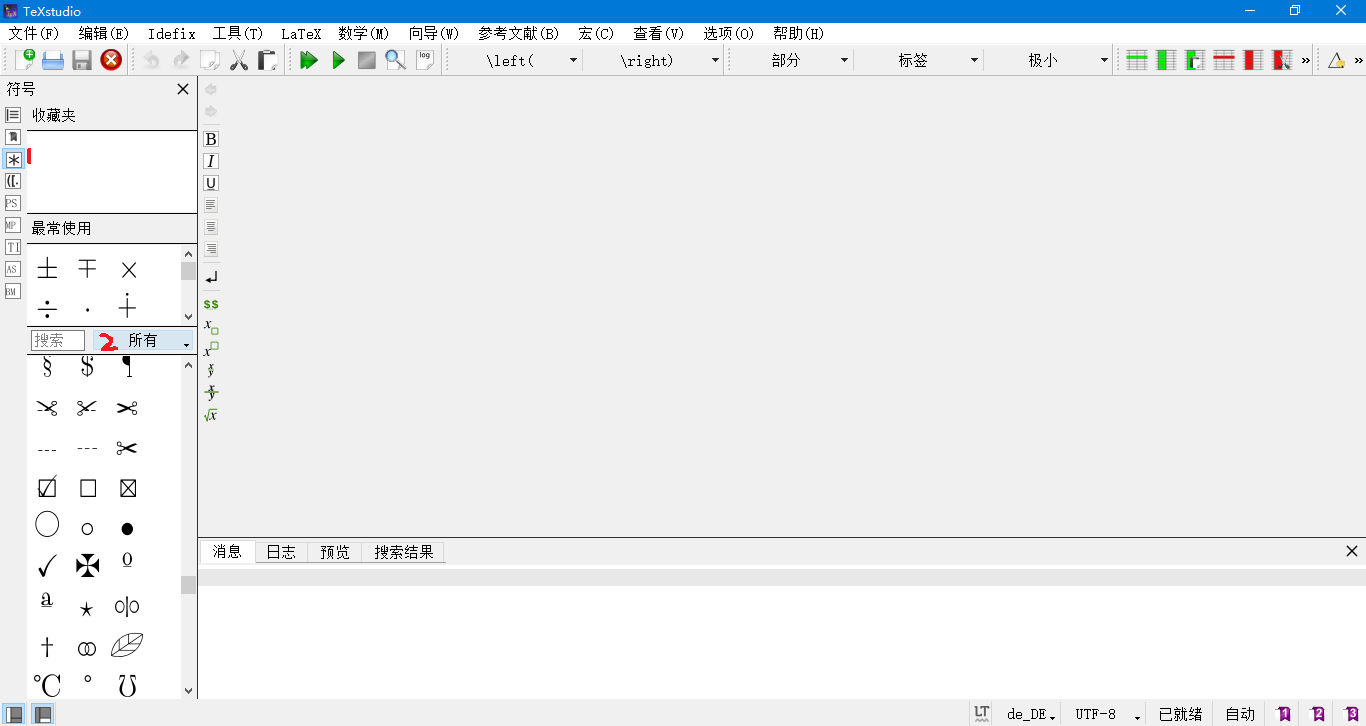
\includegraphics{https://images-cdn.shimo.im/LOSHDQ2baCooqfNu/5.png!thumbnail}
%  *
%  也可以手动输入,识别率不是特别高,可能需要多输入几次才会出来。设置如下:
%  
%  向导=\textgreater{}数学助手 手写输入完之后插入即可。
%  % \includegraphics{https://images-cdn.shimo.im/StDWQgBPj9YmY4U1/image.png!thumbnail}
%\end{faq}
%
%
%\begin{faq}{如何找到FAQs}
%  
%  \begin{enumerate}
%    \def\labelenumi{\arabic{enumi}.}
%    \setcounter{enumi}{1}
%    
%    \item
%    如何控制章节编号的深度
%  \end{enumerate}
%  
%  LaTeX 标准文档类对章节划分了层级: * 在 article 文档类里 part 为
%  0,section 为1,依此类推; * 在 report/book 文档类里 part 为-1,chapter
%  为0,section 为1,等等。
%  
%  secnumdepth 计数器控制章节编号的深度,如果章节的层级大于
%  secnumdepth,那么章节的标题、在目录和页眉页脚的标题都不编号(照常生成目录和页眉页脚),章节计数器也不计数。可以用
%  \cs{setcounter} 命令设置 secnumdepth
%  为较大的数使得层级比较深的章节也编号,如设置为4 令
%  \cs{paragraph}
%  也编号;或者设置一个较小的数以取消编号,如设置为-1 令
%  \cs{chapter}
%  不编号。后者是生成不编号的章节的一个妙招,免去了手动使用
%  \cs{addcontentsline}
%  和
%  \cs{markboth}
%  
%  的麻烦。 secnumdepth 计数器在article 文档类里默认为3(subsubsection
%  一级);在 report 和 book 文档类里默认为2 (subsection 一级)。
%  下面给出一个具体的例子:
%  
%  \begin{verbatim}
%  \documentclass{book}
%  \setcounter{secnumdepth}{4}
%  \begin{document}
%  \part{part}
%  \chapter{chapter}
%  \section{section}
%  \subsection{subsection}
%  \subsubsection{subsubsection}
%  \paragraph{paragraph}
%  \end{document}
%  \end{verbatim}
%  
%  
%控制目录页排版显示深度可以使用\setcounter{tocdepth}{2},此命令表示显示到三级标题。关于此问题的具体介绍可以参考\href{https://blog.csdn.net/RobertChenGuangzhi/article/details/50480856}{网址}。
%\end{faq}
%
%
%\begin{faq}{如何下载 arXiv 上面的 TeX 源文件}
%  
%  先访问 arXiv 上面的文章,在右边找到 Downloads -\textgreater{} Other
%  formats,点击进入下载页,点击 Download
%  source。将文件下载到本地后,重命名文件,文件后缀名是
%  .tar.gz。接下来解压缩 .tar.gz 文件,即可获得 tex 源文件。
%\end{faq}
%
%
%\begin{faq}{windows 系统下用 texstudio 打开中文编写的源文件遇到乱码怎么办}
%  
%  最简单的方法是借助 notepad++ 等编辑器将文件转码为 UTF-8。如果没有
%  noteapd++,也可以直接使用 texstudio。这里我们默认文件的编码是 GB2312。
%  首先打开文件,在 texstudio 右下角找到 encoding
%  位置的内容,有时系统显示为 ISO-8859-1。点击那里,进入 More
%  encodings,在列表中点击 GB2312,然后点击按钮 view
%  with。正常来讲,乱码应该都会消失。 接下来,继续进入 More
%  encodings,在列表中点击 UTF-8,然后点击按钮 change to。
%  经过这些操作,源文件就重新变成了 UTF-8 编码。
%\end{faq}
%
%
%\begin{faq}{69.如何在listing抄录环境中显示公式}
%  
%  有时对抄录环境中的代码进行说明时,要用显示公式,
%  这时只要进选项texcl设为true即可,或者设置mathescape~选项为true。
%  
%  \begin{verbatim}
%  \begin{lstlisting}[
%  numbers=left,
%  upquote=true,
%  basicstyle=\ttfamily,
%  texcl=true,
%  language=Python
%  ]
%  #Generates Graphs $G^{(12)} ---  G^{(17)}$
%  sGL6=['E@QW', 'EHQW', 'E@`w', 'E@]o', 'E@Rw', 'EAMw']
%  GL=[Graph(s) for s in sGL6]
%  \end{lstlisting}
%  \end{verbatim}
%  
%  % \begin{figure}
%  % \centering
%  % \includegraphics{https://images-cdn.shimo.im/LttXT6sECbcak9Qi/image.png!thumbnail}
%  % \caption{图片}
%  % \end{figure}
%  
%  \begin{verbatim}
%  \begin{lstlisting}[mathescape=true]
%  if foo
%  list= { $S_1,S_2,S_3$ }
%  \end{lstlisting}
%  \end{verbatim}
%\end{faq}
%
%
%\begin{faq}{能不能介绍一下排版试卷的方法与技巧,比如选择题,密封线设置等。}
%  
%  \begin{enumerate}
%    \def\labelenumi{\arabic{enumi}.}
%    \setcounter{enumi}{1}
%    
%    \item
%    一个文档,如何在不同部分使用不同的页眉页脚
%  \end{enumerate}
%  
%  参考 geometry 宏包的自定义命令。大概就是 \cs{newgeometry}\marg{options}
%  和\cs{restoregeometry} 以及 \cs{savegeometry}\marg{name}
%  和loadgeometry\{\}这四个命令了。具体可参见该宏包的说明文档。 3.
%  如何给中文文本加注音符号?
%  
%  xpinyin 宏包 4. 在book类文档中边注用什么宏包?边注的宽度能调整吗? 5.
%  如何使用ctex相关类或者宏包制定章节样式,目录样式?
%  
%  一言难尽啊 6. 如何给章节标题,目录列表加盒子边框? 7. 如何使用带圈数字?
%  
%  \begin{enumerate}
%    \def\labelenumi{\arabic{enumi}.}
%    \setcounter{enumi}{7}
%    
%    \item
%    如何改变列表标签样式,行距,缩进等各种相关间距?
%  \end{enumerate}
%  
%  enumitem 宏包 9. 换行与换段的区别,有几种方式?
%  
%  换行是\ 换段是
%  
%  \par
%  
%  ,或者空一行
%  
%换行与分段最大的区别在于语义上是否形成一段完整的阐述、叙述,多读两遍你写的文字,如果你觉得问题没有叙述完,那么应该用换行,反之则应该用分段。
%\end{faq}
%
%
%\begin{faq}{在使用较早版本的CTeX里面附带的 winedt 出现打不开utf8编码文档的情况,如何处理?}
%  
%  使用记事本之类文本编辑器打开,转换编码方式另存一份即可。有时候需要注意BOM问题,一般没啥问题。
%\end{faq}
%
%
%\begin{faq}{如何改变计数器样式为 中文数字 罗马数字 阿拉伯数字 拉丁字母?}
%  
%  可以通过重定义命令的方式修改默认的计数器样式,例如:
%  
%  \begin{verbatim}
%  \renewcommand{\thechapter}{\Roman{chapter}}
%  \end{verbatim}
%  
%  如上指令将章序号计数器改为大写罗马数字计数形式。
%  % \arabic\textbar{}阿拉伯数字\textbar{} :----\textbar{}:----\textbar{}
%  % \alph\textbar{}小写英文字母,数值应小于27\textbar{}
%  % \Alph\textbar{}大写英文字母,数值应小于27\textbar{}
%  % \chinese\textbar{}中文小写数字,需要调用ctex宏包\textbar{}
%  % \roman\textbar{}小写罗马数字\textbar{}
%  % \Roman\textbar{}大写罗马数字\textbar{}
%  % \fnsymbol\textbar{}脚注标识符,数值应小于10\textbar{}
%  
%  详情可以参阅刘海洋、胡伟等编写的相应书籍,也可以查阅wiki百科。 2.
%  列表环境 (enumerate/itemize/description)
%  的条目间距太大了,怎么改小一些?
%  
%  可以使用 paralist
%  宏包,它提供了一系列压缩了行间距的列表。对应的环境名称分别是
%  compactenum/compactitem/compactdesc ,也可以使用 enumitem
%  宏包修改三个列表环境的格式。 3.
%  列表的条目项内容很短,可以让他们在一行内排版么?
%  
%  可以使用 paralist 宏包,这个宏包提供了 inparenum/inparitem/inpardesc
%  环境,可以在行内输出列表内容;也可以带上 inline 选项使用 enumitem
%  宏包,可以使用带*形式的三个列表环境,即在行内输出列表内容。 4. enumerate
%  宏包修改列表标签格式很方便,但是这个宏包和 enumitem
%  宏包冲突,有什么解决办法么?
%  
%  如果只是需要使用这种短标签表示方法,利用 enumitem
%  宏包同样能够做到,只需要带上 shortlabels 选项加载 enumitem
%  宏包即可。同时,enumitem
%  宏包提供了自定义短标签名称和格式的宏命令,你也可以自己定义一些有趣的标签形式。
%  5. 如何使用带圈数字作为 enumerate 列表的标签?
%  
%  LaTeX 自带一个带圈字符的命令
%  \textcircled,不过,这个命令的排版效果非常差,几乎很少有人会直接使用。带圈数字可以通过unicode字符实现,也可通过
%  pifont 宏包中 \cs{ding} 命令实现(但是只能用到10以内的数字),甚至可以通过
%  tikz 自己绘制一个。使用带圈数字做enumerate的标签,可以通过 enumitem
%  宏包设置。这里给出一个使用 unicode 字符实现带圈数字的方法,并将其应用于
%  enumerate 的标签。
%  
%  \begin{verbatim}
%  \documentclass{article}
%  \usepackage{xeCJK,xunicode,calc}
%  \usepackage[shortlabels]{enumitem}
%  \newcommand{\Cnum}[1]{%
%  \ifnum #1<21
%  \edef\a{\the\numexpr #1+9311}
%  \else
%  \ifnum #1<36
%  \edef\a{\the\numexpr #1+12860}
%  \else
%  \ifnum #1<51
%  \edef\a{\the\numexpr #1+12941}
%  \else
%  \PackageError{your package}{Number too large}{}
%  \fi
%  \fi
%  \fi
%  {\CJKfontspec{Noto Serif CJK SC}\fontspec{Noto Serif CJK SC}\symbol\a}}
%  \SetEnumerateShortLabel{o}{\protect\Cnum{\arabic*}}
%  \begin{document}
%  \Cnum{12} \Cnum{32} \Cnum{46}
%  
%  \begin{enumerate}[o]
%  \item The first item.
%  \item The second item.
%  \item The Third One.
%  \end{enumerate}
%  \end{document}
%  \end{verbatim}
%\end{faq}
%
%
%\begin{faq}{如何给目录中的章节都带上引导点来连接页码?}
%  
%  其实级别较高的章节结构,如 book/report
%  中的chapter和arcticle中的section,是不需要这种引导点来连接页码的,有这种需求的多是受MS
%  Word 的影响。如果一定要这种引导点,可以在导言区增加这样一段代码。
%  
%  \begin{verbatim}
%  \makeatletter
%  \def\@bfdottedtocline#1#2#3#4#5{%
%  \ifnum #1>\c@tocdepth \else
%  \vskip \z@ \@plus.2\p@
%  {\leftskip #2\relax \rightskip \@tocrmarg \parfillskip -\rightskip
%  \parindent #2\relax\@afterindenttrue
%  \interlinepenalty\@M
%  \leavevmode \bfseries
%  \@tempdima #3\relax
%  \advance\leftskip \@tempdima \null\nobreak\hskip -\leftskip
%  {#4}\normalfont\nobreak
%  \leaders\hbox{$\m@th
%  \mkern \@dotsep mu\hbox{.}\mkern \@dotsep
%  mu$}\hfill
%  \nobreak
%  \hb@xt@\@pnumwidth{\hfil\normalfont \normalcolor #5}%
%  \par}%
%  \fi}
%  \renewcommand*\l@section{\@bfdottedtocline{0}{0em}{1.5em}}
%  \makeatother
%  \end{verbatim}
%  
%  当然,最后一句应根据实际的文档类型来重定义\l@chapter或\l@section.
%\end{faq}
%
%
%\begin{faq}{如何临时切换页面大小?}
%  
%  \begin{enumerate}
%    \def\labelenumi{\arabic{enumi}.}
%    \setcounter{enumi}{1}
%    
%    \item
%    没有编号的章节标题如何添加到目录里?
%  \end{enumerate}
%  
%  使用
%  \begin{verbatim}
%  \addcontentsline{toc}{⟨level⟩}{⟨title⟩}
%  \end{verbatim}
%  
%  ;举个例子:
%  \begin{verbatim}
%  \section*{译者序}\addcontentsline{toc}{section}{译者序}
%  \end{verbatim}
%  
%  这样在目录中译者序是没有编号的,对应等级是section,标题是译者序
%  参考:《lshort》目录章节 3. 怎样定义 第几页/共几页 的页码样式?
%  
%  可以调用末页标签宏包lastpage,并将页码设置如下:
%  
%  \begin{verbatim}
%  第 \thepage 页 / 共 \pageref{LastPage} 页
%  \end{verbatim}
%  
%  如果不想调用这个宏包,还可以自己DIY,虽然ugly,但是可以达到目的 ):
%  在文档末尾设置一个标签,例如在 \verb|\end{doucument}| 前加一句 
%  \verb|\label{AllPage}|,然后将页码设置为:
%  
%  \begin{verbatim}
%  第 \thepage 页 / 共 \pageref{AllPage} 页
%  \end{verbatim}
%  
%  \begin{enumerate}
%    \def\labelenumi{\arabic{enumi}.}
%    \setcounter{enumi}{3}
%    
%    \item
%    超链接如何断行?
%  \end{enumerate}
%  
%  先写
%  
%  \begin{verbatim}
%  \PassOptionsToPackage{hyphens}{url}
%  \end{verbatim}
%  
%  再写
%  
%  \begin{verbatim}
%  \usepackage{hyperref}
%  \end{verbatim}
%\end{faq}
%
%
%\begin{faq}{在使用较早版本的CTeX里面附带的winedt出现打不开utf8编码文档的情况,如何处理?}
%  
%  使用记事本之类文本编辑器打开,转换编码方式另存一份即可。有时候需要注意BOM问题,一般没啥问题。
%  2. 如何在axmath转换代码到texstudio?
%  
%  点击下图中第10个按钮,即可将数学公式转换为LaTeX代码,复制即可。
%  % \includegraphics{https://images-cdn.shimo.im/oMh77ZPr7iIsh2tB/image.png!thumbnail}
%  3.
%  双栏文档中,如何可以让左边先写完,然后再切换到右边,而不是左右一样长?
%  
%  如果是采用文档类 twocolumn
%  选项实现的双栏模式,正文的排版就是先将左边排完,再从右边开始排。而采用
%  multicol 宏包的 muticols 环境则是左右两边底部对齐的。 4.
%  如何输入中文破折号?
%  
%  输入法输入咯,英文的破折号 --- 用于中文不合适。 5.
%  \cs{input} 和 \cs{include} 有何区别? * \cs{include}
%  在读入文件之前会另起一页。\cs{input}
%  命令纯粹是把文件里的内容插入 * \cs{include}不可用于导言区
%\end{faq}
%
%
%\begin{faq}{subfiles有什么用?}
%  
%  \begin{enumerate}
%    \def\labelenumi{\arabic{enumi}.}
%    \setcounter{enumi}{1}
%    
%    \item
%    ~如何使用latexmk编译文档?
%    \item
%    定理环境要怎么使用?
%    \item
%    算法环境如何使用?
%    \item
%    在lstlisting环境中如何输出破折号?
%    \item
%    minted里面tab键为什么会输出成\^{}\^{}T,如何解决?
%    \item
%    一段代码粘贴到texstudio里面就没有了缩进,如何解决?
%    \item
%    在LaTeX或Tikz中,能否输入随机且字数随机可控的文字?
%    \item
%    如何输入罗马数字等?
%    \item
%    如何在等号中插入问号?
%  \end{enumerate}
%  
%  \begin{verbatim}
%  \stackrel{?}{=}.
%  \end{verbatim}
%\end{faq}
%
%
%\begin{faq}{如何在插入的图片上标记引注?}
%  
%  \begin{enumerate}
%    \def\labelenumi{\arabic{enumi}.}
%    \setcounter{enumi}{1}
%    
%    \item
%    如何让一个很长很长的字符串(中间不带空格)自动换行?
%    \item
%    \cs{bf} \cs{sf} \cs{it} \cs{sl} 这些命令都很短小,为什么不建议继续使用了?
%    \item
%    如何自动化打包 LaTeX
%    文档发送给别人以确保宏包、字体是完整的,便于他人顺利编译、减少麻烦。
%    \item
%    如何编译网站上下载的他人的模板,一般是不知道对应的编译器应该选择什么,还有编译顺序是什么,希望在提供模板的同时说明应该如何编译。
%    \item
%    我以book文档类为基础新写一个文档类,book文档类的选项会自动适用于我新建的文档类么?
%    \item
%    \cs{def} 和 \cs{newcommand}
%    有什么区别,我创建新命令的时候究竟应该用哪个?
%    \item
%    怎样创建一个带*的命令?
%    \item
%    ~类似 \verb|\macro[<option1>][<option2>]{<arg>}|
%    这样的宏命令,当我只使用一个可选参数时,LaTeX
%    把它看做哪个参数?LaTeX会自动判断么?
%    \item
%    \cs{newcommand}
%    创建的命令,仅有第一个命令可以成为可选参数,如果我想创建具有两个可选参数的命令,应该如何去写?
%    \item
%    有些命令的参数是使用( ) 扩起来的,这类命令是如何定义的?
%    \item
%    我想新建一个带有可选参数的命令,可选参数的缺省值与必选参数值一样,这样的命令如何创建?
%    \item
%    想用minted包写文档,怕别人用不来不会设置-shell --escepe咋办
%    \item
%    .latex如何给整个页面加边框? \# 四、介绍公式的常见问题。
%  \end{enumerate}
%\end{faq}
%
%
%\begin{faq}{\cs{ldots} 与...有什么区别?}
%  
%  重定义的难度不同、造成的间距也不同。推荐使用 \cs{ldots}。 见
%  \url{https://www.zhihu.com/question/27589739/answer/37255728}
%  
%  \begin{enumerate}
%    \def\labelenumi{\arabic{enumi}.}
%    \setcounter{enumi}{1}
%    
%    \item
%    如何让长公式自动断行?
%  \end{enumerate}
%  
%  
%长公式自动断行要看情况,如果是在行内模式,合理使用空格,一般可以在二元运算符处断行,如果是行间模式,推荐使用align类环境,在需要断行处添加
%  \ 手动断行。 3. 公式希腊字符如何加粗?
%  
%  希腊字母没有粗体,可以选择合适的数学字体。 可以使用 bm
%  宏包将希腊字母加粗。
%\end{faq}
%
%
%\begin{faq}{极限符号下面有两个趋近该怎么写}
%  
%  直接给出例子:
%  
%  \begin{verbatim}
%  \documentclass{article}
%  \begin{document}
%  \[ \lim_{n\to\infty\atop m\to\infty} \]
%  \end{document}
%  \end{verbatim}
%  
%  或者使用 \cs{substack},代码如下:
%  
%  \begin{verbatim}
%  \documentclass{article}
%  \usepackage{amsmath}
%  \begin{document}
%  \[ \lim_{\substack{n\to\infty\\ m\to\infty}} \]
%  \end{document}
%  \end{verbatim}
%  
%  效果如下:
%  % \includegraphics{https://images-cdn.shimo.im/FCY4A1SeBIcwBCGT/双重极限.PNG!thumbnail}
%\end{faq}
%
%
%\begin{faq}{怎样在 LaTeX 中输入引号}
%  
%  左引号用 `(键盘1旁边那个键),右引号用 `。双引号也一样,``''。
%  
%中文条件下可以直接用中文引号(这个与编码方式和中文支持方式有关的),会有自动配对(这个和编辑器以及输入法有关的),但是如果需要用到不配对引号的情况,需要使用通用方法。
%\end{faq}
%
%
%\begin{faq}{align环境默认是居中对齐吗?我在使用时,发现公式开始是居中的,后来却一直靠右断对齐,这是什么原因?}
%  
%  \sout{align 默认靠右对齐,所以通常加 \&
%    符号,让代码左对齐。验证一下以下代码:}
%  
%  \begin{verbatim}
%  \begin{align}
%  & \nabla \times H = J,\\
%  & \nabla \times E = - \partial _t B,\\
%  & \nabla \cdot B = 0.
%  \end{align}
%  \end{verbatim}
%  
%  再试试把 \& 去掉什么样。
%  align采用的是奇偶对齐的方式,第一列右对齐,第二列左对齐,就这样右左右左依此类推,两列之间用\&分隔。
%\end{faq}
%
%
%\begin{faq}{中英文标点使用规则不是很明白,尤其在公式环境里,字体和间距差别都比较大。怎样才能让正文和公式的标点统一(形状和间隔)?}
%  
%  详见:
%  
%\url{https://link.zhihu.com/?target=http\%3A//www.moe.gov.cn/ewebeditor/uploadfile/2015/01/13/20150113092346124.pdf}
%  在导言区加类似命令可实现全文替换:
%  
%  \begin{verbatim}
%  \catcode`\。=\active\newcommand{。}{. }
%  \end{verbatim}
%  
%  或者使用 xeCJK 宏包的字符映射功能,调用 fullwidth-stop
%  这一映射文件,将中文空心句号映射为实心句点:
%  
%  \begin{verbatim}
%  \documentclass{article}
%  \usepackage{xeCJK}
%  \setCJKmainfont[Mapping= fullwidth-stop]{STSong}
%  \begin{document}
%  句号。
%  \end{document}
%  \end{verbatim}
%  
%  \begin{enumerate}
%    \def\labelenumi{\arabic{enumi}.}
%    \setcounter{enumi}{1}
%    
%    \item
%    公式如何居左对齐,居右对齐?
%  \end{enumerate}
%  
%  公式居左对齐在基础文档类中由 fleqn
%  选项控制,选择该选项后,正文公式均居左对齐,至于居右对齐,嗯,我没见过这么奇怪的格式。
%  3. 公式之后解释公式符号的文字,通常是 ``符号 ------ 解释''
%  这样的格式,我希望这段文字的格式是按破折号对齐,并且解释文字折行后悬挂缩进,怎样实现这样的格式?
%  
%  方法很多,可以列表,可以align等环境。 这里给出一个使用自定义列表的例子:
%  
%  \begin{verbatim}
%  \usepackage{ifthen}
%  \newcounter{qlst}
%  \newenvironment{EqDesc}[2][式中]{%
%  \begin{list}{}
%  {%
%  \usecounter{qlst}
%  \settowidth{\labelwidth}{#1,#2\ --- \ }
%  \setlength{\labelsep}{0pt}
%  \setlength{\leftmargin}{\labelwidth}
%  \setlength{\rightmargin}{0em}
%  \setlength{\parsep}{0ex}
%  \setlength{\itemsep}{0ex}
%  \setlength{\itemindent}{0em}
%  \setlength{\listparindent}{0em}
%  \renewcommand{\makelabel}[1]{\stepcounter{qlst}\ifthenelse{\value{qlst}>1}{\hfill ##1\ --- \ 
%  }{#1,\hfill ##1\ --- \ }}
%  }}%
%  {\end{list}}%
%  \end{verbatim}
%  
%  \env{EqDesc} 
%  环境有两个参数,第一个为可选参数,是解释公式符号前的引导词,默认是“式中”,第二个参数是样本符号,可以选择一个列表中宽度最大的符号。条目
%   \cs{item} 有一个可选参数(实际使用是必选参数),内容是要说明的符号。使用如下:
%  
%  \begin{verbatim}
%  \[ a^2+b^2=c^2 \]
%  \begin{EqDesc}[其中]{$a$}
%  \item[$a$] 三角形的一条直角边;
%  \item[$b$] 三角形的另一条直角边;
%  \item[$c$] 三角形的斜边。
%  \end{EqDesc}
%  \end{verbatim}
%\end{faq}
%
%
%\begin{faq}{行内公式的情况下如何让sum prod这些运算符的上下标在头上和脚下?}
%  
%  这样处理行内公式的上下标会导致段落行距不整齐,不符合 LaTeX
%  的审美。如果彻底放弃审美,可以使用 \cs{limits} 命令,如:
%  
%  \begin{verbatim}
%  $\sum\limits_{i=1}^n \quad
%  \prod\limits_\epsilon$
%  \end{verbatim}
%\end{faq}
%
%
%\begin{faq}{如何将积分的上限标放在积分号的上下两侧?}
%  
%  积分号的上下限放置在积分号的右侧是英美国家和 LaTeX
%  的排版习惯,通常无需处理。如果你很确定需要按照 ISO 80000-2:2009 或者 GB
%  3102.11-93 的规定排版积分号,可以:
%  
%  
%  
%  % \begin{enumerate}
%  % % \def\labelenumi{\arabic{enumi}.}
%  % % \setcounter{enumi}{1}
%  % %
%  % \item
%  %   在调用 amsmath 宏包时添加 intlimits 选项;
%  % \item
%  %   \texttt{\def\int\{\intop\}}
%  % \item
%  %   如果使用 unicode-math 宏包,
%  % \end{enumerate}
%  \begin{verbatim}
%  \removenolimits{%
%  \int\iint\iiint\iiiint\oint\oiint\oiiint
%  \intclockwise\varointclockwise\ointctrclockwise\sumint
%  \intbar\intBar\fint\cirfnint\awint\rppolint
%  \scpolint\npolint\pointint\sqint\intlarhk\intx
%  \intcap\intcup\upint\lowint
%  }
%  \end{verbatim}
%\end{faq}
%
%
%\begin{faq}{如何自定义数学运算符,然后让下标放在脚下?}
%  
%  借助 amsmath 包的
%  \cs{DeclareMathOperator*} 命令即可(需要注意加不加*是有区别的)。例如
%  
%  \begin{verbatim}
%  \DeclareMathOperator*{\esssup}{ess\,sup}
%  \end{verbatim}
%\end{faq}
%
%
%\begin{faq}{在数学公式中,编辑等式时,每一行需要等号和等号对其,这时使用了
%    \cs{begin}\Arg{displaymath},
%    \cs{begin}\Arg{split} 环境,但是呢,这些整体都是居中的,我想让式子靠左,怎么实现呢?}
%  
%  \begin{enumerate}
%    \def\labelenumi{\arabic{enumi}.}
%    \setcounter{enumi}{1}
%    
%    \item
%    行列式变换过程中,我们一般是在中间的箭头上表示出变换的方式,如何才能在长箭头上打出多行内容?
%    \item
%    如何输出反斜杠?
%  \end{enumerate}
%  
%  \begin{verbatim}
%  \textbackslash \verb|\|
%  \end{verbatim}
%  
%  \begin{enumerate}
%    \def\labelenumi{\arabic{enumi}.}
%    \setcounter{enumi}{3}
%    
%    \item
%    对equation环境下的公式、图片编号按章节、小节进行重新定义 \#
%    五、参考文献篇
%  \end{enumerate}
%\end{faq}
%
%
%\begin{faq}{参考文献中的特殊字符或字母}
%  
%  \begin{enumerate}
%    \def\labelenumi{\arabic{enumi}.}
%    \setcounter{enumi}{1}
%    
%    \item
%    BibTeX 不理解的作者列表
%  \end{enumerate}
%  
%  BibTeX 只支持三种姓名格式: * First von Last * von Last, First * von
%  Last, Jr, First
%  
%  多个姓名之间必须使用``and''连接,如
%  
%  \begin{verbatim}
%  author = {Knuth, Donald E. and Lamport, Leslie},
%  \end{verbatim}
%  
%  \begin{enumerate}
%    \def\labelenumi{\arabic{enumi}.}
%    \setcounter{enumi}{2}
%    
%    \item
%    BibTeX 排序和名字前缀
%    \item
%    BibTeX 中的大写字母
%  \end{enumerate}
%  
%  英文标题中常使用的大小写方式有:
%\end{faq}
%
%
%\begin{faq}{Title case:
%    句首字母大写,并且除冠词、连词和短介词以外的词首字母大写,这里说的``短''介词一般指不超过
%    4 个字母的介词。比如``The Quick Brown Fox Jumps over the Lazy
%    Dog'';}
%  
%  \begin{enumerate}
%    \def\labelenumi{\arabic{enumi}.}
%    \setcounter{enumi}{1}
%    
%    \item
%    Sentence case:
%    句首字母和一些专有名词的首字母大写,同普通的英文句子大小写方式一样,如``The
%    quick brown fox jumps over the lazy dog''。
%  \end{enumerate}
%  
%  BibTeX 根据 bst 样式文件可以将题名保留原大小写,或转为 sentence
%  case。所以用户在 bib 数据库中著录标题的正确方式是,统一使用 title
%  case,并将需要专有名词用大括号括起来。
%  
%  \begin{verbatim}
%  title = {Finite Element Methods for {Maxwell's} Equations},
%  \end{verbatim}
%  
%  
%注意尽量避免将一个词中个别字母用大括号括起来,如``\{M\}axwell's'',这可能会导致字母的间距有问题,建议将整个词括起来,如``\{Maxwell's\}''。
%\end{faq}
%
%
%\begin{faq}{如何选择参考文献的风格}
%  
%  参考文献的风格一般是期刊或会议模板指定 bst
%  的,作者应仔细阅读投稿要求和模板使用说明,根据规定使用合适的
%  bst。通常有以下方式:
%  
%  1. 在文档中声明 `
%  \begin{verbatim}
%  \bibliographystyle{ieeetran}
%  \end{verbatim}
%  
%  2. 在模板的文档类选项中使用合适的参数,如
%  \begin{verbatim}
%  \documentclass[authoryear]{ustcthesis}。
%  \end{verbatim}
%\end{faq}
%
%
%\begin{faq}{BibTeX 参考文献数据库}
%  
%  BibTeX 的 bib 文件是一个记录已阅文献的数据库,但是通常不建议手动编译 bib 文件,建议:
%  1. 使用 JabRef 或 Zotero 等文献管理工具导出 bib 文件创
%  2. 使用 [Google Scholar](https://scholar.google.com/) 或 [Bing 
%  学术](https://cn.bing.com/academic)导出 bib 条目建
%  3. 创建参考文献风格
%  
%  BibTeX 的风格文件 bst 是使用一种后缀语言写的代码,如果对编程能力比较自信的话,可以阅读 BibTeX 的文档 
%  btxdoc 和 btxhak,btxbst.doc 文件提供了标准 bst 风格的代码注释,另外还可以阅读 ttb 和 The LaTeX 
%  Companion 等资料。
%  
%  如果不习惯 bst 的编程语言,可以使用 custom-bib 工具,在命令行下运行latex 
%  makebst,回答一系列问题生成自己的bst。
%  
%  另外还可以考虑使用 biblatex,它提供更方便的接口用于自定义参考文献格式。
%  
%  4. 参考文献中的数字格式
%  
%  参考文献表中的数字格式是由 \@biblabel 控制的,可以通过重定义该命令来修改格式。比如将数字修改为左对齐:
%  ```
%  \makeatletter
%  \renewcommand\@biblabel[1]{[#1]\hfill}
%  \makeatother
%  ```
%  
%  5. BibTeX文献条目列表
%  
%  科技论文通常要求参考文献表中的文献必须在正文中引用,但是在某些特殊情况下仅需要列出 bib 
%  数据库中的文献,可以使用 \nocite{*} 命令列出调用的bib中所有条目,或者使用类似\nocite{ref1,ref2,ref3}命令列出需要显示的条目。
%  
%  6. 制作参考文献的HTML
%  7. BibTeX中的多字母缩写
%  8. 多个参考文献表
%  
%  natbib宏包与Donald Arseneau和Niel 
%  
%Kempson编写的chapterbib宏包兼容,该宏包允许在一个文档内有多个独立的参考文献列表。通常用法是一本书的各章有独立的参考文献列表,尤其是在各章由不同作者独立编写时。
%  
%  9. 同一位置多文献引用
%  
%  只需要将多篇文献的bibkey用英文半角逗号分隔写在一个cite指令的选项里即可。如:
%  ```
%  \cite{knuth84,lamport86}
%  ```
%  10. 非英文参考文献条目
%  
%  什么叫非英文参考文献条目?是指bibkey么?一般不建议用中文,处理好编码格式,无殊。
%  中文的参考文献条目,与英文条目并没有什么差别,只是注意编码。目前处理中文推荐用xelatex 编译 utf8 
%  编码的文件。因此中文的 bib 条目也应该用 utf8 编码。
%  11. **BibTeX**** 文献手写很困难,有没有什么工具能够生成?**
%  
%  多数时候,我们无需自己手写 BibTeX 文献条目。从 
%  
%[https://scholar.google.com/](https://scholar.google.com/)、[https://academic.microsoft.com/](https://academic.microsoft.com/)、
%   [https://cn.bing.com/academic?mkt=zh-CN](https://cn.bing.com/academic?mkt=zh-CN) 
%  或者期刊、数据库的网站上都能够导出 BibTeX 文献条目。
%  老牌的文献管理软件 EndNote 也支持生成 BibTeX 格式的数据库,详情见 
%  官网[https://endnote.com/](https://endnote.com/)。
%  开源软件 JabRef 甚至支持 BibTeX 文献条目的导入、导出和管理,详情见 
%  官网[http://www.jabref.org/](http://www.jabref.org/)。
%  Zetero 使用起来也非常方便,详情见官网 [https://www.zotero.org/](https://www.zotero.org/)。
%  谷歌学术、知网、百度学术、万方数据库等在线数据库也是可以支持导出 .bib 文件的,至于哪家的数据条目更全,就得你自己去甄别了。
%\end{faq}
%
%
%\begin{faq}{如何使用 BibTeX 排版参考文献}
%  
%  * 准备一份 BibTeX 数据库,假设数据库文件名为 books.bib,和 LaTeX 源代码一般位于同一个目录下。
%  * 在源代码中添加必要的命令,如 \bibliographystyle{abbrv},\bibliography{books}。假设源代码名为 
%  demo.tex。其中,\bibliographystyle 设定参考文献的格式。\bibliography 告诉系统使用哪个数据库和参考文献列在哪个位置。
%  * 写好了以上两个文件之后,我们就可以开始编译了。例如在命令行中执行以下命令
%  \begin{verbatim}
%  xelatex demo
%  bibtex demo
%  xelatex demo
%  xelatex demo
%  \end{verbatim}
%  
%  
%或者选择一个可以自动检测是否有参考文献的编辑器,如果有,它会自动执行以上四个命令,但是有时候会遇到检测不到的情况,这时你只需要清理一下辅助文件即可。
%\end{faq}
%
%
%\begin{faq}{如何将参考文献条目录入到正文中}
%  
%  理工科类论文很少用。
%\end{faq}
%
%
%\begin{faq}{bib文件的重建}
%  
%  用文本编辑器如Notepad++, Sublime Text或WinEdt或专门文献管理软件JabRef,BibDesk等创建文件,改名为 
%  ref.bib 文件,往里头添加参考文献目录。参考如下:
%  % ![图片](https://images-cdn.shimo.im/VKQ8uAycksg1zPlo/image.png!thumbnail)
%  在.bib文件中,可以采用 TeXStudio 提供的参考文献格式,在自行修改内容
%  % ![图片](https://images-cdn.shimo.im/0OgCsRQoufMTDJ75/1.png!thumbnail)
%  上面的类型有两种选择 BibTeX 和 BibLaTeX ,后者的选择更为广泛。
%  参考文献一般不自己书写,而是有可以直接导入。
%  一般直接 Google 学术搜索出来的文献或者引用知网,如下:
%  % ![图片](https://images-cdn.shimo.im/L1fAEZmW9tYDVTYT/VRI1FEC62J_C6_QSK_P0_0.png!thumbnail)
%  点击上图红圈的引号->
%  % ![图片](https://images-cdn.shimo.im/N8tFzuXsCM8rOPjF/image.png!thumbnail)
%  在点击最左侧的 BibTeX ->
%  % ![图片](https://images-cdn.shimo.im/81Z6BGei8ycQf1uK/image.png!thumbnail)
%  将其复制黏贴到你的 ref.bib 文件中即可。
%  在知网上的文献查询需要下载安装如下软件:
%  % ![图片](https://images-cdn.shimo.im/ZsikCVGdjGIKBqSN/image.png!thumbnail)
%  两个都装好了之后,该软件需要自行注册登陆使用。
%  然后打开知网,会看到如下:
%  % ![图片](https://images-cdn.shimo.im/DVEoaSyHJKwmbSjH/2.png!thumbnail)
%  右上角红圈圈到的就是为浏览器安装的 Zotero Connector插件,在此需要打开 Zotero 
%  
%软件,点击之后显示下图,选择需要的文献。![图片](https://images-cdn.shimo.im/w4eu1WOehS05gJ0g/image.png!thumbnail)
%  然后 Zotero 软件如下显示
%  % ![图片](https://images-cdn.shimo.im/VFUjYs5MvKQz522e/image.png!thumbnail)
%  然后文件->导出文献库->导出格式 BibTeX  确定保存生成的bib文件,可以将这个 bib 
%  文件中的参考文献全部复制黏贴到你的 ref.bib 
%  文件中,也可以单独作为一个新的bib文件,在正文区则需要添加多个bib文件就可以,用命令 
%  \bibliography{test,ref},多个bib文件用逗号分隔即可。同时为引用的参考文献需要命令 \nocite{*} 来将未引用的文件全部排版出来。
%  注:百度学术、万方数据库等也支持导出 .bib 文件。
%\end{faq}
%
%
%\begin{faq}{如何减少参考文献条目行间距}
%  
%  文献条目间距为 \cs{itemsep},默认值4.5pt plus 2pt minus
%  1pt,可通过指令\cs{addtolength}\Arg{\cs{itemsep}}\marg{距离}调整。
%  
%  2. 按照章节分开参考文献条目
%  
%  可看看chapterbib宏包。
%  3. 引文的排序及压缩
%  
%  这个取决于使用的宏包,常用的natbib宏包可以使用sort或者 \verb|sort&compress| 选项激活相应的排序或排序并压缩功能。
%  4. 引文列表排序
%  
%  这个取决于bst,一般模板都有指定的bst。
%  5. BibTeX中过长的字符串
%  6. 按照“unsrt”规则的目录重排序
%  7. BibTeX参考文献中的URL
%  
%  调用url或者xurl宏包即可正常使用url,也可以看看href宏包。
%  8. 基于Plain TeX的BibTeX的使用
%  9. 常用的biblatex参考文献样式
%  
%  
%  biblatex除了可以应用自带的标准样式外,还可以使用其他作者提供的第三方样式,这里介绍一些常用的样式:
%  * 国外常用
%  * APA
%  * MLA
%  * 国内
%  * GB7714-2015
%  % 样式名|用法|对应的bibtex样式|作者介绍|样式说明|
%  % :----:|:----:|:----:|:----:|:----:|
%  % trad-plain|`\usepackage[style=trad-plain]{biblatex}`|plain|MarcoDaniel and 
%  
%%%MoritzWemheuer,后者是biblatex维护者之一|将引文按字母顺序排序,比较次序为作者姓氏、出版年份和题名,如果不能顺序,将以在正文中的引用顺序为准。|
%  % trad-unsrt|`\usepackage[style=trad-unsrt]{biblatex}`|unsrt|MarcoDaniel and 
%  %MoritzWemheuer|按照在正文中引用文献的先后顺序排列文献,其排版格式与trad-plain基本相同|
%  % trad-alpha|`\usepackage[style=trad-alpha]{biblatex}`|alpha|MarcoDaniel and 
%  
%%%MoritzWemheuer|用文献的作者姓氏前三个字母加出版年份的后两位数作为文献序号,如果出现相同的序号,则会根据排序结果在序号后追加字母以示区别,排序方法和排版格式与trad-plain相同|
%  % trad-abbrv|`\usepackage[style=trad-abbrv]{biblatex}`|abbrv|MarcoDaniel and 
%  %MoritzWemheuer|将文献中作者名和月份名的拼写改为缩写, 显得文献信息紧凑简洁, 
%  %其排序方法和排版格式与trad-plain相同|
%  % ieee|`\usepackage[style=ieee]{biblatex}`|IEEEtran|Joseph Wright,biblatex 
%  %维护者之一|国际电气电子工程师协会IEEE期刊文献格式|
%  % apa|`\usepackage[style=apa]{biblatex}`|apalike|Philip Kime,biblatex 作者之一|American 
%  %Psychological Association 的文献格式|
%  % Chicago|`\usepackage{biblatex-chicago}`|Chicago|David Fussner|for the Chicago Manual of Style|
%  % iso-numeric|`\usepackage[style=iso-numeric]{biblatex}`| |Michal Hoftich|ISO690 international 
%  %standard numeric system|
%  % iso-iso-authoryear|`\usepackage[style=iso-iso-authoryear]{biblatex}`| |Michal Hoftich|ISO690 
%  %international standard nameanddate system,so-called Harvard style|
%  % gb7714-2015|`\usepackage[style=gb7714-2015]{biblatex}`|gbt7714-unsrt.bst by 
%  %zepinglee|hushidong|中文文献著录标准 GB/T 7714-2015 顺序编码制|
%  % gb7714-2015ay|`\usepackage[style=gb7714-2015ay]{biblatex}`|gbt7714-plain.bst by 
%  %zepinglee|hushidong|中文文献著录标准 GB/T 7714-2015 著者年份制|
%  % caspervector|`\usepackage[style=caspervector]{biblatex}`| |Casper vector|一种中文文献格式|
%  % nature|`\usepackage[style=nature]{biblatex}`| |Joseph Wright|for Nature|
%  % science|`\usepackage[style=science]{biblatex}`| |Joseph Wright|for Science|
%  % chem-acs|`\usepackage[style=chem-acs]{biblatex}`| |Joseph Wright|covers most American 
%%Chemistry 
%  %Society journals|
%  % chem-angew|`\usepackage[style=chem-angew]{biblatex}`| |Joseph Wright|covers Angewandte Chemie 
%  %Chemistry–A European Journal.|
%  % chem-biochem|`\usepackage[style=chem-biochem]{biblatex}`| |Joseph Wright|covers Biochemistry 
%  %and asmallnumber of other American Chemistry Society journals|
%  % chem-rsc|`\usepackage[style=chem-rsc ]{biblatex}`| |Joseph Wright|covers all Royal Society of 
%  %Chemistry journals|
%  % phys|`\usepackage[style=phys]{biblatex}`| |Joseph Wright|for AIP and APS|
%  % nejm|`\usepackage[style=nejm]{biblatex}`| |MarcoDaniel|for New England Journal of Medicine|
%  % mla|`\usepackage[style=mla]{biblatex}`| |James Clawson|for Modern Language Association|
%  % authortitle-dw|`\usepackage[style=authortitle-dw]{biblatex}`| |Dominik Waßenhoven|for 
%  %Humanities|
%  % footnote-dw|`\usepackage[style=footnote-dw]{biblatex}`| |Dominik Waßenhoven|for Humanities|
%\end{faq}
%
%
%\begin{faq}{使用超链接,如何去除颜色边框?}
%  
%  直接在引用 hyperref 宏包的时候使用以下命令之一
%  \begin{verbatim}
%  \usepackage[hidelinks]{hyperref}
%  \usepackage[colorlinks]{hyperref}
%  \end{verbatim}
%  
%  第一种方法是隐藏链接,即隐藏颜色和边框。
%  第二种方法是用不同颜色来替换默认的边框强调超链接的方式,但是这种方法会使得链接具有不同的颜色。如果需要设置各种链接的颜色可以参考
%   hyprref 
%  
%的说明文档,值得庆幸的是,该宏包已经有了一个[中文翻译版](https://github.com/latexstudio/LaTeXPackages-CN/blob/master/hyperref/hyperref-zh-cn.pdf)。
%\end{faq}
%
%
%\begin{faq}{参考文献列表行距如何设置?}
%  
%  设置好文献条目间距 \cs{itemsep} 即可。
%\end{faq}
%
%
%\begin{faq}{参考文献编号如何左对齐,右对齐?}
%\end{faq}
%
%
%\begin{faq}{插入参考文献列表有几种方式?如何定义其样式?如何定义正文引用样式?}
%\end{faq}
%
%
%\begin{faq}{不同 journal 给出的 bibtex 文件格式不一致,如何批量快速格式化多个 .bib 文件}

